\documentclass{report}
\usepackage[utf8]{inputenc}
\usepackage[T1]{fontenc}
\usepackage[swissgerman]{babel}
\usepackage[left=2cm,right=1.5cm,top=1.5cm,bottom=1.5cm]{geometry}
\usepackage{amssymb}
\usepackage{ragged2e}
\usepackage{titlesec}
\usepackage{booktabs}
\usepackage{svg}
\usepackage{transparent}
\usepackage{float}
\usepackage{hyperref}
\usepackage[many]{tcolorbox}
\usepackage{epigraph}
\usepackage{listings}

\lstloadlanguages{Java,Ruby}
\lstdefinestyle{fmo}{
  keywordstyle=\color{blue},
  identifierstyle=\bfseries\color{black},
  frame=single,
  basicstyle=\footnotesize\ttfamily,
  showstringspaces=false,
  keepspaces=true,
}
\lstset{style=fmo}

\setsvg{inkscape=inkscape -z -D,svgpath=__src/svg/}

\setlength\parindent{0pt}
\linespread{1.3}

\titleformat{\chapter}[display]
{\normalfont\huge\bfseries}{\chaptertitlename\ \thechapter}{20pt}{\Huge}
\titlespacing*{\chapter}{0pt}{0pt}{40pt}

%\renewcommand{\labelenumi}{\alph{enumi}.}

\newcommand{\pro}[1]{\item [pro]#1}
\newcommand{\con}[1]{\item [con]#1}

\newtcolorbox{caveat}[1][]{
  breakable,
  freelance,
  title=CAVEAT: #1,
  colback=white,
  colbacktitle=white,
  coltitle=black,
  fonttitle=\bfseries,
  bottomrule=0pt,
  boxrule=0pt,
  colframe=white,
  overlay unbroken and first={
    \draw[red!75!black,line width=3pt]
    ([xshift=5pt]frame.north west) -- 
    (frame.north west) -- 
    (frame.south west);
    \draw[red!75!black,line width=3pt]
    ([xshift=-5pt]frame.north east) -- 
    (frame.north east) -- 
    (frame.south east);
  },
  overlay unbroken app={
    \draw[red!75!black,line width=3pt,line cap=rect]
    (frame.south west) -- 
    ([xshift=5pt]frame.south west);
    \draw[red!75!black,line width=3pt,line cap=rect]
    (frame.south east) -- 
    ([xshift=-5pt]frame.south east);
  },
  overlay middle and last={
    \draw[red!75!black,line width=3pt]
    (frame.north west) -- 
    (frame.south west);
    \draw[red!75!black,line width=3pt]
    (frame.north east) -- 
    (frame.south east);
  },
  overlay last app={
    \draw[red!75!black,line width=3pt,line cap=rect]
    (frame.south west) --
    ([xshift=5pt]frame.south west);
    \draw[red!75!black,line width=3pt,line cap=rect]
    (frame.south east) --
    ([xshift=-5pt]frame.south east);
  },
}

\newtcolorbox{additional}[1][]{
  breakable,
  freelance,
  title=Additional Resources: #1,
  colback=white,
  colbacktitle=white,
  coltitle=black,
  fonttitle=\bfseries,
  bottomrule=0pt,
  boxrule=0pt,
  colframe=white,
  overlay unbroken and first={
    \draw[green!75!black,line width=3pt]
    ([xshift=5pt]frame.north west) -- 
    (frame.north west) -- 
    (frame.south west);
    \draw[green!75!black,line width=3pt]
    ([xshift=-5pt]frame.north east) -- 
    (frame.north east) -- 
    (frame.south east);
  },
  overlay unbroken app={
    \draw[green!75!black,line width=3pt,line cap=rect]
    (frame.south west) -- 
    ([xshift=5pt]frame.south west);
    \draw[green!75!black,line width=3pt,line cap=rect]
    (frame.south east) -- 
    ([xshift=-5pt]frame.south east);
  },
  overlay middle and last={
    \draw[green!75!black,line width=3pt]
    (frame.north west) -- 
    (frame.south west);
    \draw[green!75!black,line width=3pt]
    (frame.north east) -- 
    (frame.south east);
  },
  overlay last app={
    \draw[green!75!black,line width=3pt,line cap=rect]
    (frame.south west) --
    ([xshift=5pt]frame.south west);
    \draw[green!75!black,line width=3pt,line cap=rect]
    (frame.south east) --
    ([xshift=-5pt]frame.south east);
  },
}

\title{POSA 1 - HS2015}

\author{Valentin \textsc{Meier}\\\\Vorlage von Felix \textsc{Morgner}}

\date{\today}

\begin{document}

\maketitle
\clearpage
\vspace*{\fill}
  \epigraph{Sometimes the questions are complicated and the answers are simple.}{Dr. Seuss}
\vfill
\clearpage

\setcounter{tocdepth}{0}
\tableofcontents

\chapter{Layers}

\section{Summary}
Das Layer Pattern hilft Applikationen zu strukturieren, welche in Gruppen von Teilaufgaben zerteilt werden können so dass, jede Gruppe auf einem bestimmten Abstraktionslevel ist.
\section{Context}
Ein grosses System das Zerlegung benötigt.

\section{Problem}
Ein grosses System mit Low- und Highlevel Problemen hat zu wenig Struktur. Die Highlevel-Probleme bauen dabei auf den Lowlevel-Problemen auf. Es ist schwer Wartbar und die Aufgaben und Grenzen zwischen den Komponenten sind ungenau.

Ein mögliches Beispiel für ein solches System ist ein Netzwerk. Dabei ist ein Lowlevel-Problem: \textit{"Wie bringe ich Daten von A nach B?"} und ein Highlevel-Problem: \textit{"Wie ordne ich verschiedene Pakete einer logischen Session zu?"}

\section{Solution}
Das System wird in beliebig viele Layer aufgeteilt. Die Layer bauen aufeinander auf, wobei der höchste Layer den höchsten Abstraktionsgrad hat. Alle Komponenten mit dem selben Abstrationsgrad befinden sich auf dem selben Layer. Jedem Layer werden bestimmte Aufgaben zugewiesen. Er nutzt jeweils die Services des eins tieferen Layers. \\\\
Bei vielen Komponenten pro Layer wird je Layer ein Interface Objekt definiert welches mit den anderen Layern kommuniziert. Meist wird aus einem Request (Zugriff von Oben nach Unten) mehrere je tiefer der Request in den Layern nach unten wandert. Das Umgekehrte gilt bei einer Notification (Zugriff von Unten nach Oben).
Die folgenden Schritte beschreiben einen schrittweisen Ansatz zur Definition einer Layer Architektur. Dies ist nicht immer die beste Lösung. Es sind auch nicht alle Schritte zwingend notwendig. Vorgehen:
\begin{enumerate}
	\item Abstraktionskriterien definieren (Wie die Layer sich abgrenzen)
	\item Anzahl Abstraktionslevel definieren
	\item Layers benennen und Tasks zuteilen
	\item Services pro Layer spezifizieren
	\item 1.-4. zur Verfeinerung wiederholen
	\item Ein Interface pro Layer definieren, eventuell Facade Pattern anwenden
	\item Layer im Innern strukturieren (Bridge/Strategy Pattern)
	\item Kommunikation zwischen benachbarten Layern spezifizieren
	\item Benachbarte Layer entkuppeln (Bsp. One-Way Coupling/Retour mit Callbacks)
	\item Error Handling Strategie entwickeln. Entweder im Layer behandeln oder an den nächst höheren weitergeben. Faustregel:Am besten am tiefstmöglichen Layer behandeln.
\end{enumerate}
Es gibt noch zwei weitere Varianten des Layer Pattern:
\begin{description}
	\item[Relaxed Layered System] Layer können Services aller unterliegenden Layer benutzen. Mehr Flexibilität und Performance, jedoch schlechtere Wartbarkeit.
	\item[Layering through inheritance] Für OO-Systeme. Lower Layer als base classes. Höhere Layer erben von diesen. So können höhere Layer Funktionalität von tieferen ihren Bedürfnissen anpassen.
\end{description}

\subsection{Structure}

\begin{figure}[H]
  \centering
  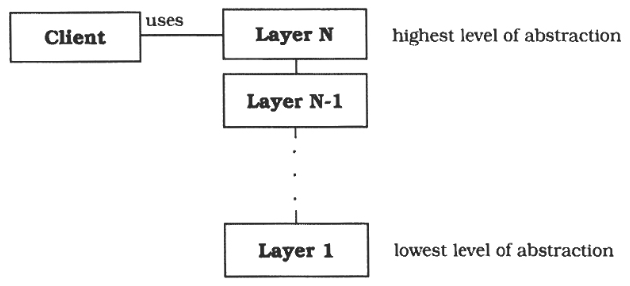
\includegraphics[width=0.8\textwidth]{figures/00-layers-1}
  \caption{Illustration des Layer-Patterns}
\end{figure}

\section{Consequences}
\begin{itemize}
    \pro{Wiederverwendbarkeit von Layern}
    \pro{Austauschbarkeit von Layern}
    \pro{Support für Standardisierung}
    \pro{Dependencies bleiben lokal}
    \con{Tiefere Effizienz}
    \con{Mehr Aufwand}
    \con{Schwierigkeit beim bestimmen der Granularität der Layer}
    \con{Jeder Layer-Übergang schmälert die Performance}
\end{itemize}

\section{Known Uses}
\begin{itemize}
	\item OSI Protocol Stack 
	\item Virtual Machines
	\item APIs
	\item Information Systems
	\item Windows NT
\end{itemize}

\section{Relationships}
\begin{itemize}
	\item \textit{Composite Message} beschreibt eine objekt-orientierte Verschachtelung von Nachrichten, welche durch die Schichten transportiert werden. Eine Composite Message ist ein Paket, welches aus header, payload und eingebetteten Paketen besteht.
	\item \textit{Mikrokernel Architecture} kann als spezialisierte Layer-Architektur angesehen werden.
\end{itemize}

\section{Exam Questions}
\begin{itemize}
  \item Behauptung: Etwas zu bottom-up dekouplung in layer? (Lösung)
    \item Frage: Welches GOF Pattern hilft bei der definierung von Interfaces im Layers Pattern? (Facace Pattern)
\end{itemize}

\chapter{Pipes and Filters}

\section{Summary}
Das "Pipes and Filters" Pattern bietet eine Struktur für Systeme die einen Stream von Daten verarbeiten, dabei wird jeder Verarbeitungsschritt als eine Filterkomponente dargestellt. Die Daten bewegen sich durch Pipes zwischen benachbarten Filtern.  
\section{Context}
Durch das "Pipies and Filters" Pattern werden folgende Forces adressiert: 
\begin{itemize}
	\item Zukünftige Systemerweiterungen sollten durch Austausch oder Neuordnung von Verarbeitungsschritten möglich sein
	\item Kleine Verarbeitungsschritte sind einfacher wiederverwendbar als grosse
	\item Nicht benachbarte Verarbeitungsschritte sollen keine Informationen teilen
	\item Es gibt verschiedene Quellen von Input Daten
	\item Es soll möglich sein Schlussresultate auf verschiedene Arten zu sichern
	\item Explizites Speichern von Zwischenresultate durch User ist fehleranfällig
	\item Man will die Möglichkeit nicht verwerfen, die Arbeitsschritte parallel zu verarbeiten
\end{itemize}


\section{Problem}
Gegeben ist ein System welches einen Stream von Daten verarbeiten muss. Das System wird von mehreren Entwicklern implementiert. Ausserdem lässt sich die generelle Aufgabe des Systems leicht in mehrere Teilaufgaben unterteilen, und die Wahrscheinlichkeit ist hoch, dass sich die Requirements ändern. Die Frage ist nun wie ein solches System designt werden soll damit mehrere Entwickler daran arbeiten können und flexibel auf Änderungen an den Requirements reagiert werden kann.
\section{Solution}
Mittels dem "Pipies and Filters" Pattern werden die Arbeitsschritte eines Systems in mehrere sequentiell verarbeitete Schritte unterteilt. Die Schritte sind durch den Data Flow durch das System verbunden, das heisst, die Output Daten eines Schrittes sind die Input Daten des nächsten. Jeder Arbeitsschritt wird als Filter Komponente implementiert. Ein Filter konsumiert und übermittelt inkrementell. Die Daten Source, die Filter und der Daten "Sink" werden durch sogenannte Pipes verbunden. 

\subsection{Structure}
Filter sind die Verarbeitungseinheiten einer Pipeline. Ein Filter hat drei Aufgaben:
\begin{enumerate}
	\item Anreichern von Daten durch Berechnungen und hinzufügen von Informationen
	\item Verfeinern von Daten durch Konzentration oder Extraktion von Daten
	\item Transformieren von Daten durch Übermittlung in einer anderen Repräsentation
\end{enumerate}
Ein Filter kann durch verschiedene Events ausgelöst werden:
\begin{itemize}
	\item Der darauffolgende Filter pullt die Output Daten
	\item Der vorangehende Filter pushed die Input Daten
	\item Üblicherweise pulling von Input Daten und pushen von Output Daten in einem Loop
\end{itemize}
Bei den ersten beiden Methoden handelt es sich um passive Filter, weil sie darauf warten getriggert zu werden. Bei der dritten Methode handelt es sich um einen aktiven Filter.

%\begin{figure}[H]
%  \centering
%  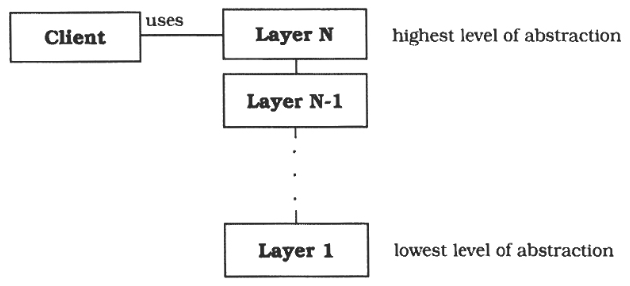
\includegraphics[width=0.8\textwidth]{figures/00-layers-1}
%  \caption{Illustration des Layer-Patterns}
%\end{figure}

\section{Consequences}
\begin{itemize}
    \pro{Keine Speicherung von Zwischenresultaten notwendig, jedoch weiterhin möglich}
    \pro{Flexibilität durch Filteraustausch}
    \pro{Flexibilität durch Neuordnung der Filterreihenfolge}
    \pro{Wiederverwendbarkeit von Filterkomponenten}
    \pro{Schnelles erstellen von Prototypen von Pipelines}
    \pro{Effizienz durch Parallelverarbeitung}
    \con{Teilen von Informationen über den State ist teuer}
    \con{Effizienzsteigerung durch Parallelverarbeitung ist meist eine Illusion}
    \con{Daten Transformations Overhead}
    \con{Error Handling}
    
\end{itemize}

\section{Known Uses}
\begin{itemize}
	\item UNIX
	\item CMS Pipelines
	\item LASSPTools
\end{itemize}

\section{Relationships}
\begin{itemize}
	\item \textit{Layers Pattern} Besser geeignet für Systeme welche zuverlässige Operationen benötigen, da es einfacher ist Error Handling zu implementieren
\end{itemize}

\section{Exam Questions}
\begin{itemize}
  \item Behauptung: dies ist eine Behauptung? (Lösung)
    \item Frage: Dies ist eine Frage? (Lösung)
\end{itemize}


\clearpage
\vspace*{\fill}
\begin{center}
    { \huge \bfseries :wq }
\end{center}
\vfill
\clearpage


\end{document}
